% Options for packages loaded elsewhere
\PassOptionsToPackage{unicode}{hyperref}
\PassOptionsToPackage{hyphens}{url}
\PassOptionsToPackage{dvipsnames,svgnames,x11names}{xcolor}
%
\documentclass[
  letterpaper,
  DIV=11,
  numbers=noendperiod]{scrartcl}

\usepackage{amsmath,amssymb}
\usepackage{iftex}
\ifPDFTeX
  \usepackage[T1]{fontenc}
  \usepackage[utf8]{inputenc}
  \usepackage{textcomp} % provide euro and other symbols
\else % if luatex or xetex
  \usepackage{unicode-math}
  \defaultfontfeatures{Scale=MatchLowercase}
  \defaultfontfeatures[\rmfamily]{Ligatures=TeX,Scale=1}
\fi
\usepackage{lmodern}
\ifPDFTeX\else  
    % xetex/luatex font selection
\fi
% Use upquote if available, for straight quotes in verbatim environments
\IfFileExists{upquote.sty}{\usepackage{upquote}}{}
\IfFileExists{microtype.sty}{% use microtype if available
  \usepackage[]{microtype}
  \UseMicrotypeSet[protrusion]{basicmath} % disable protrusion for tt fonts
}{}
\makeatletter
\@ifundefined{KOMAClassName}{% if non-KOMA class
  \IfFileExists{parskip.sty}{%
    \usepackage{parskip}
  }{% else
    \setlength{\parindent}{0pt}
    \setlength{\parskip}{6pt plus 2pt minus 1pt}}
}{% if KOMA class
  \KOMAoptions{parskip=half}}
\makeatother
\usepackage{xcolor}
\setlength{\emergencystretch}{3em} % prevent overfull lines
\setcounter{secnumdepth}{-\maxdimen} % remove section numbering
% Make \paragraph and \subparagraph free-standing
\ifx\paragraph\undefined\else
  \let\oldparagraph\paragraph
  \renewcommand{\paragraph}[1]{\oldparagraph{#1}\mbox{}}
\fi
\ifx\subparagraph\undefined\else
  \let\oldsubparagraph\subparagraph
  \renewcommand{\subparagraph}[1]{\oldsubparagraph{#1}\mbox{}}
\fi


\providecommand{\tightlist}{%
  \setlength{\itemsep}{0pt}\setlength{\parskip}{0pt}}\usepackage{longtable,booktabs,array}
\usepackage{calc} % for calculating minipage widths
% Correct order of tables after \paragraph or \subparagraph
\usepackage{etoolbox}
\makeatletter
\patchcmd\longtable{\par}{\if@noskipsec\mbox{}\fi\par}{}{}
\makeatother
% Allow footnotes in longtable head/foot
\IfFileExists{footnotehyper.sty}{\usepackage{footnotehyper}}{\usepackage{footnote}}
\makesavenoteenv{longtable}
\usepackage{graphicx}
\makeatletter
\def\maxwidth{\ifdim\Gin@nat@width>\linewidth\linewidth\else\Gin@nat@width\fi}
\def\maxheight{\ifdim\Gin@nat@height>\textheight\textheight\else\Gin@nat@height\fi}
\makeatother
% Scale images if necessary, so that they will not overflow the page
% margins by default, and it is still possible to overwrite the defaults
% using explicit options in \includegraphics[width, height, ...]{}
\setkeys{Gin}{width=\maxwidth,height=\maxheight,keepaspectratio}
% Set default figure placement to htbp
\makeatletter
\def\fps@figure{htbp}
\makeatother

\usepackage{booktabs}
\usepackage{longtable}
\usepackage{array}
\usepackage{multirow}
\usepackage{wrapfig}
\usepackage{float}
\usepackage{colortbl}
\usepackage{pdflscape}
\usepackage{tabu}
\usepackage{threeparttable}
\usepackage{threeparttablex}
\usepackage[normalem]{ulem}
\usepackage{makecell}
\usepackage{xcolor}
\usepackage{wrapfig}
\KOMAoption{captions}{tableheading}
\makeatletter
\makeatother
\makeatletter
\makeatother
\makeatletter
\@ifpackageloaded{caption}{}{\usepackage{caption}}
\AtBeginDocument{%
\ifdefined\contentsname
  \renewcommand*\contentsname{Table of contents}
\else
  \newcommand\contentsname{Table of contents}
\fi
\ifdefined\listfigurename
  \renewcommand*\listfigurename{List of Figures}
\else
  \newcommand\listfigurename{List of Figures}
\fi
\ifdefined\listtablename
  \renewcommand*\listtablename{List of Tables}
\else
  \newcommand\listtablename{List of Tables}
\fi
\ifdefined\figurename
  \renewcommand*\figurename{Figure}
\else
  \newcommand\figurename{Figure}
\fi
\ifdefined\tablename
  \renewcommand*\tablename{Table}
\else
  \newcommand\tablename{Table}
\fi
}
\@ifpackageloaded{float}{}{\usepackage{float}}
\floatstyle{ruled}
\@ifundefined{c@chapter}{\newfloat{codelisting}{h}{lop}}{\newfloat{codelisting}{h}{lop}[chapter]}
\floatname{codelisting}{Listing}
\newcommand*\listoflistings{\listof{codelisting}{List of Listings}}
\makeatother
\makeatletter
\@ifpackageloaded{caption}{}{\usepackage{caption}}
\@ifpackageloaded{subcaption}{}{\usepackage{subcaption}}
\makeatother
\makeatletter
\@ifpackageloaded{tcolorbox}{}{\usepackage[skins,breakable]{tcolorbox}}
\makeatother
\makeatletter
\@ifundefined{shadecolor}{\definecolor{shadecolor}{rgb}{.97, .97, .97}}
\makeatother
\makeatletter
\makeatother
\makeatletter
\makeatother
\ifLuaTeX
  \usepackage{selnolig}  % disable illegal ligatures
\fi
\IfFileExists{bookmark.sty}{\usepackage{bookmark}}{\usepackage{hyperref}}
\IfFileExists{xurl.sty}{\usepackage{xurl}}{} % add URL line breaks if available
\urlstyle{same} % disable monospaced font for URLs
\hypersetup{
  pdftitle={Tests},
  colorlinks=true,
  linkcolor={blue},
  filecolor={Maroon},
  citecolor={Blue},
  urlcolor={Blue},
  pdfcreator={LaTeX via pandoc}}

\title{Tests}
\author{}
\date{}

\begin{document}
\maketitle
\ifdefined\Shaded\renewenvironment{Shaded}{\begin{tcolorbox}[interior hidden, enhanced, breakable, boxrule=0pt, sharp corners, frame hidden, borderline west={3pt}{0pt}{shadecolor}]}{\end{tcolorbox}}\fi

Read in data

Make a table

\begin{table}

\end{table}

See \textbf{?@tbl-table1} for details.

Now try for the kable version:

\begin{table}

\end{table}

\begin{verbatim}
-- Attaching core tidyverse packages ------------------------ tidyverse 2.0.0 --
v dplyr     1.1.4     v readr     2.1.5
v forcats   1.0.0     v stringr   1.5.1
v ggplot2   3.5.0     v tibble    3.2.1
v lubridate 1.9.3     v tidyr     1.3.1
v purrr     1.0.2     
-- Conflicts ------------------------------------------ tidyverse_conflicts() --
x dplyr::filter() masks stats::filter()
x dplyr::lag()    masks stats::lag()
i Use the conflicted package (<http://conflicted.r-lib.org/>) to force all conflicts to become errors
here() starts at /Users/samharper/git/bhet-report


Attaching package: 'kableExtra'


The following object is masked from 'package:dplyr':

    group_rows


Rows: 12 Columns: 6
-- Column specification --------------------------------------------------------
Delimiter: ","
chr (3): Pollutant, Category, Effect
dbl (3): Estimate, CI_low, CI_upper

i Use `spec()` to retrieve the full column specification for this data.
i Specify the column types or set `show_col_types = FALSE` to quiet this message.
\end{verbatim}

\hypertarget{tbl-table3}{}
\begin{table}
\caption{\label{tbl-table3}Summary: Numeric variables using kableExtra }\tabularnewline

\centering
\begin{tabular}{llrrrrrr}
\toprule
\multicolumn{2}{c}{ } & \multicolumn{3}{c}{DiD} & \multicolumn{3}{c}{Adjusted DiD} \\
\cmidrule(l{3pt}r{3pt}){3-5} \cmidrule(l{3pt}r{3pt}){6-8}
  &   & Estimate & LL & UL & Estimate & LL & UL\\
\midrule
\addlinespace[0.3em]
\multicolumn{8}{l}{\textbf{Air pollution}}\\
\hspace{1em} & Black carbon & -0.45 & -1.85 & 0.96 & -0.45 & -1.81 & 0.92\\
\cmidrule{2-8}
\multirow[t]{-2}{*}[1\dimexpr\aboverulesep+\belowrulesep+\cmidrulewidth]{\raggedright\arraybackslash Personal} & PM2.5 & 2.14 & -31.39 & 35.67 & 7.00 & -21.28 & 35.28\\
\cmidrule{1-8}
\hspace{1em} & Daily & -37.97 & -74.79 & -1.14 & -31.17 & -63.98 & 1.64\\
\cmidrule{2-8}
\multirow[t]{-2}{*}[1\dimexpr\aboverulesep+\belowrulesep+\cmidrulewidth]{\raggedright\arraybackslash Indoor} & Seasonal & -38.97 & -55.29 & -22.64 & -37.72 & -54.01 & -21.44\\
\cmidrule{1-8}
\hspace{1em} & Daily & -0.11 & -5.86 & 5.64 & -1.73 & -9.26 & 5.81\\
\cmidrule{2-8}
\multirow[t]{-2}{*}[1\dimexpr\aboverulesep+\belowrulesep+\cmidrulewidth]{\raggedright\arraybackslash Outdoor} & Seasonal & 3.14 & -3.10 & 9.38 & 0.36 & -6.27 & 6.99\\
\bottomrule
\end{tabular}
\end{table}

Another DiD table

\begin{table}
\centering
\begin{tabular}{llcccc}
\toprule
\multicolumn{2}{c}{ } & \multicolumn{2}{c}{DiD} & \multicolumn{2}{c}{Adjusted DiD*} \\
\cmidrule(l{3pt}r{3pt}){3-4} \cmidrule(l{3pt}r{3pt}){5-6}
  &   & Estimate & (95\% CI) & Estimate & (95\% CI)\\
\midrule
\addlinespace[0.3em]
\multicolumn{6}{l}{\textbf{Air pollution (µg/m3)}}\\
\hspace{1em} & PM2.5 & -2.09 & (-29.38, 25.2) & 1.95 & (-23.34, 27.23)\\
\cmidrule{2-6}
\multirow[t]{-2}{*}[1\dimexpr\aboverulesep+\belowrulesep+\cmidrulewidth]{\raggedright\arraybackslash Personal} & Black carbon & -0.46 & (-1.73, 0.81) & -0.43 & (-1.67, 0.81)\\
\cmidrule{1-6}
\hspace{1em} & Daily & -19.10 & (-60.56, 22.35) & -15.38 & (-53.54, 22.78)\\
\cmidrule{2-6}
\multirow[t]{-2}{*}[1\dimexpr\aboverulesep+\belowrulesep+\cmidrulewidth]{\raggedright\arraybackslash Indoor} & Seasonal & -35.11 & (-59.36, -10.85) & -36.27 & (-60.26, -12.29)\\
\cmidrule{1-6}
\hspace{1em} & Daily & -0.11 & (-5.86, 5.64) & -1.73 & (-9.26, 5.81)\\
\cmidrule{2-6}
\multirow[t]{-2}{*}[1\dimexpr\aboverulesep+\belowrulesep+\cmidrulewidth]{\raggedright\arraybackslash Outdoor} & Seasonal & 3.14 & (-3.1, 9.38) & 0.36 & (-6.27, 6.99)\\
\cmidrule{1-6}
\addlinespace[0.3em]
\multicolumn{6}{l}{\textbf{Respiratory (percentage points)}}\\
\hspace{1em} & Any symptom & -7.38 & (-13.98, -0.77) & -7.86 & (-14.63, -1.09)\\
\cmidrule{2-6}
\hspace{1em} & Coughing & -1.59 & (-6.41, 3.23) & -1.98 & (-6.8, 2.84)\\
\cmidrule{2-6}
\hspace{1em} & Phlegm & -1.22 & (-5.58, 3.15) & -1.82 & (-6.34, 2.69)\\
\cmidrule{2-6}
\hspace{1em} & Wheezing attacks & -0.22 & (-3.97, 3.52) & -0.14 & (-3.85, 3.57)\\
\cmidrule{2-6}
\hspace{1em} & Trouble breathing & -4.98 & (-11.81, 1.84) & -4.62 & (-11.59, 2.35)\\
\cmidrule{2-6}
\multirow[t]{-6}{*}[5\dimexpr\aboverulesep+\belowrulesep+\cmidrulewidth]{\raggedright\arraybackslash Self-reported (pp)} & Chest trouble & -6.63 & (-12.51, -0.76) & -6.36 & (-12.14, -0.59)\\
\bottomrule
\multicolumn{6}{l}{\rule{0pt}{1em}\textsuperscript{*} Footnote A}\\
\end{tabular}
\end{table}

See Table~\ref{tbl-table3} for more.

\begin{table}
\centering
\begin{tabular}{llcccc}
\toprule
\multicolumn{2}{c}{ } & \multicolumn{2}{c}{DiD} & \multicolumn{2}{c}{Adjusted DiD*} \\
\cmidrule(l{3pt}r{3pt}){3-4} \cmidrule(l{3pt}r{3pt}){5-6}
  &   & Estimate & (95\% CI) & Estimate & (95\% CI)\\
\midrule
\addlinespace[0.3em]
\multicolumn{6}{l}{\textbf{Blood pressure (mmHg)}}\\
\hspace{1em} & Brachial & -0.79 & (-2.63, 1.04) & -1.40 & (-3.31, 0.51)\\
\cmidrule{2-6}
\multirow[t]{-2}{*}[1\dimexpr\aboverulesep+\belowrulesep+\cmidrulewidth]{\raggedright\arraybackslash Systolic BP} & Central & -1.04 & (-2.82, 0.73) & -1.56 & (-3.40, 0.28)\\
\cmidrule{1-6}
\hspace{1em} & Brachial & -1.29 & (-2.62, 0.04) & -1.60 & (-2.96, -0.25)\\
\cmidrule{2-6}
\multirow[t]{-2}{*}[1\dimexpr\aboverulesep+\belowrulesep+\cmidrulewidth]{\raggedright\arraybackslash Diastolic BP} & Central & -1.35 & (-2.66, 0.04) & -1.66 & (-2.97, -0.34)\\
\cmidrule{1-6}
\hspace{1em} & Brachial & 0.50 & (-0.71, 1.70) & 0.21 & (-1.00, 1.41)\\
\cmidrule{2-6}
\multirow[t]{-2}{*}[1\dimexpr\aboverulesep+\belowrulesep+\cmidrulewidth]{\raggedright\arraybackslash Pulse Pressure} & Central & 0.31 & (-0.85, 1.46) & 0.10 & (-1.01, 1.20)\\
\cmidrule{1-6}
\hspace{1em} & Pulse pressure & 0.10 & (-0.12, 1.40) & 0.00 & (-1.20, 1.20)\\
\cmidrule{2-6}
\multirow[t]{-2}{*}[1\dimexpr\aboverulesep+\belowrulesep+\cmidrulewidth]{\raggedright\arraybackslash BP Amplification x10} & Systolic BP & 0.20 & (-0.20, 0.50) & 0.10 & (-0.20, 0.40)\\
\cmidrule{1-6}
\addlinespace[0.3em]
\multicolumn{6}{l}{\textbf{Respiratory}}\\
\hspace{1em} & Any symptom & -7.38 & (-13.98, -0.77) & -7.86 & (-14.63, -1.09)\\
\cmidrule{2-6}
\hspace{1em} & Coughing & -1.59 & (-6.41, 3.23) & -1.98 & (-6.8, 2.84)\\
\cmidrule{2-6}
\hspace{1em} & Phlegm & -1.22 & (-5.58, 3.15) & -1.82 & (-6.34, 2.69)\\
\cmidrule{2-6}
\hspace{1em} & Wheezing attacks & -0.22 & (-3.97, 3.52) & -0.14 & (-3.85, 3.57)\\
\cmidrule{2-6}
\hspace{1em} & Trouble breathing & -4.98 & (-11.81, 1.84) & -4.62 & (-11.59, 2.35)\\
\cmidrule{2-6}
\multirow[t]{-6}{*}[5\dimexpr\aboverulesep+\belowrulesep+\cmidrulewidth]{\raggedright\arraybackslash Self-reported (pp)} & Chest trouble & -6.63 & (-12.51, -0.76) & -6.36 & (-12.14, -0.59)\\
\cmidrule{1-6}
\hspace{1em}Measured & FeNO (ppb) & 0.17 & (-2.24, 2.58) & 0.55 & (-2.13, 3.13)\\
\bottomrule
\multicolumn{6}{l}{\rule{0pt}{1em}\textit{Note: } pp = percentage points, ppb = parts per billion}\\
\multicolumn{6}{l}{\rule{0pt}{1em}\textsuperscript{*} List of adjustments...}\\
\end{tabular}
\end{table}

```

\newpage

\begin{figure}

{\centering 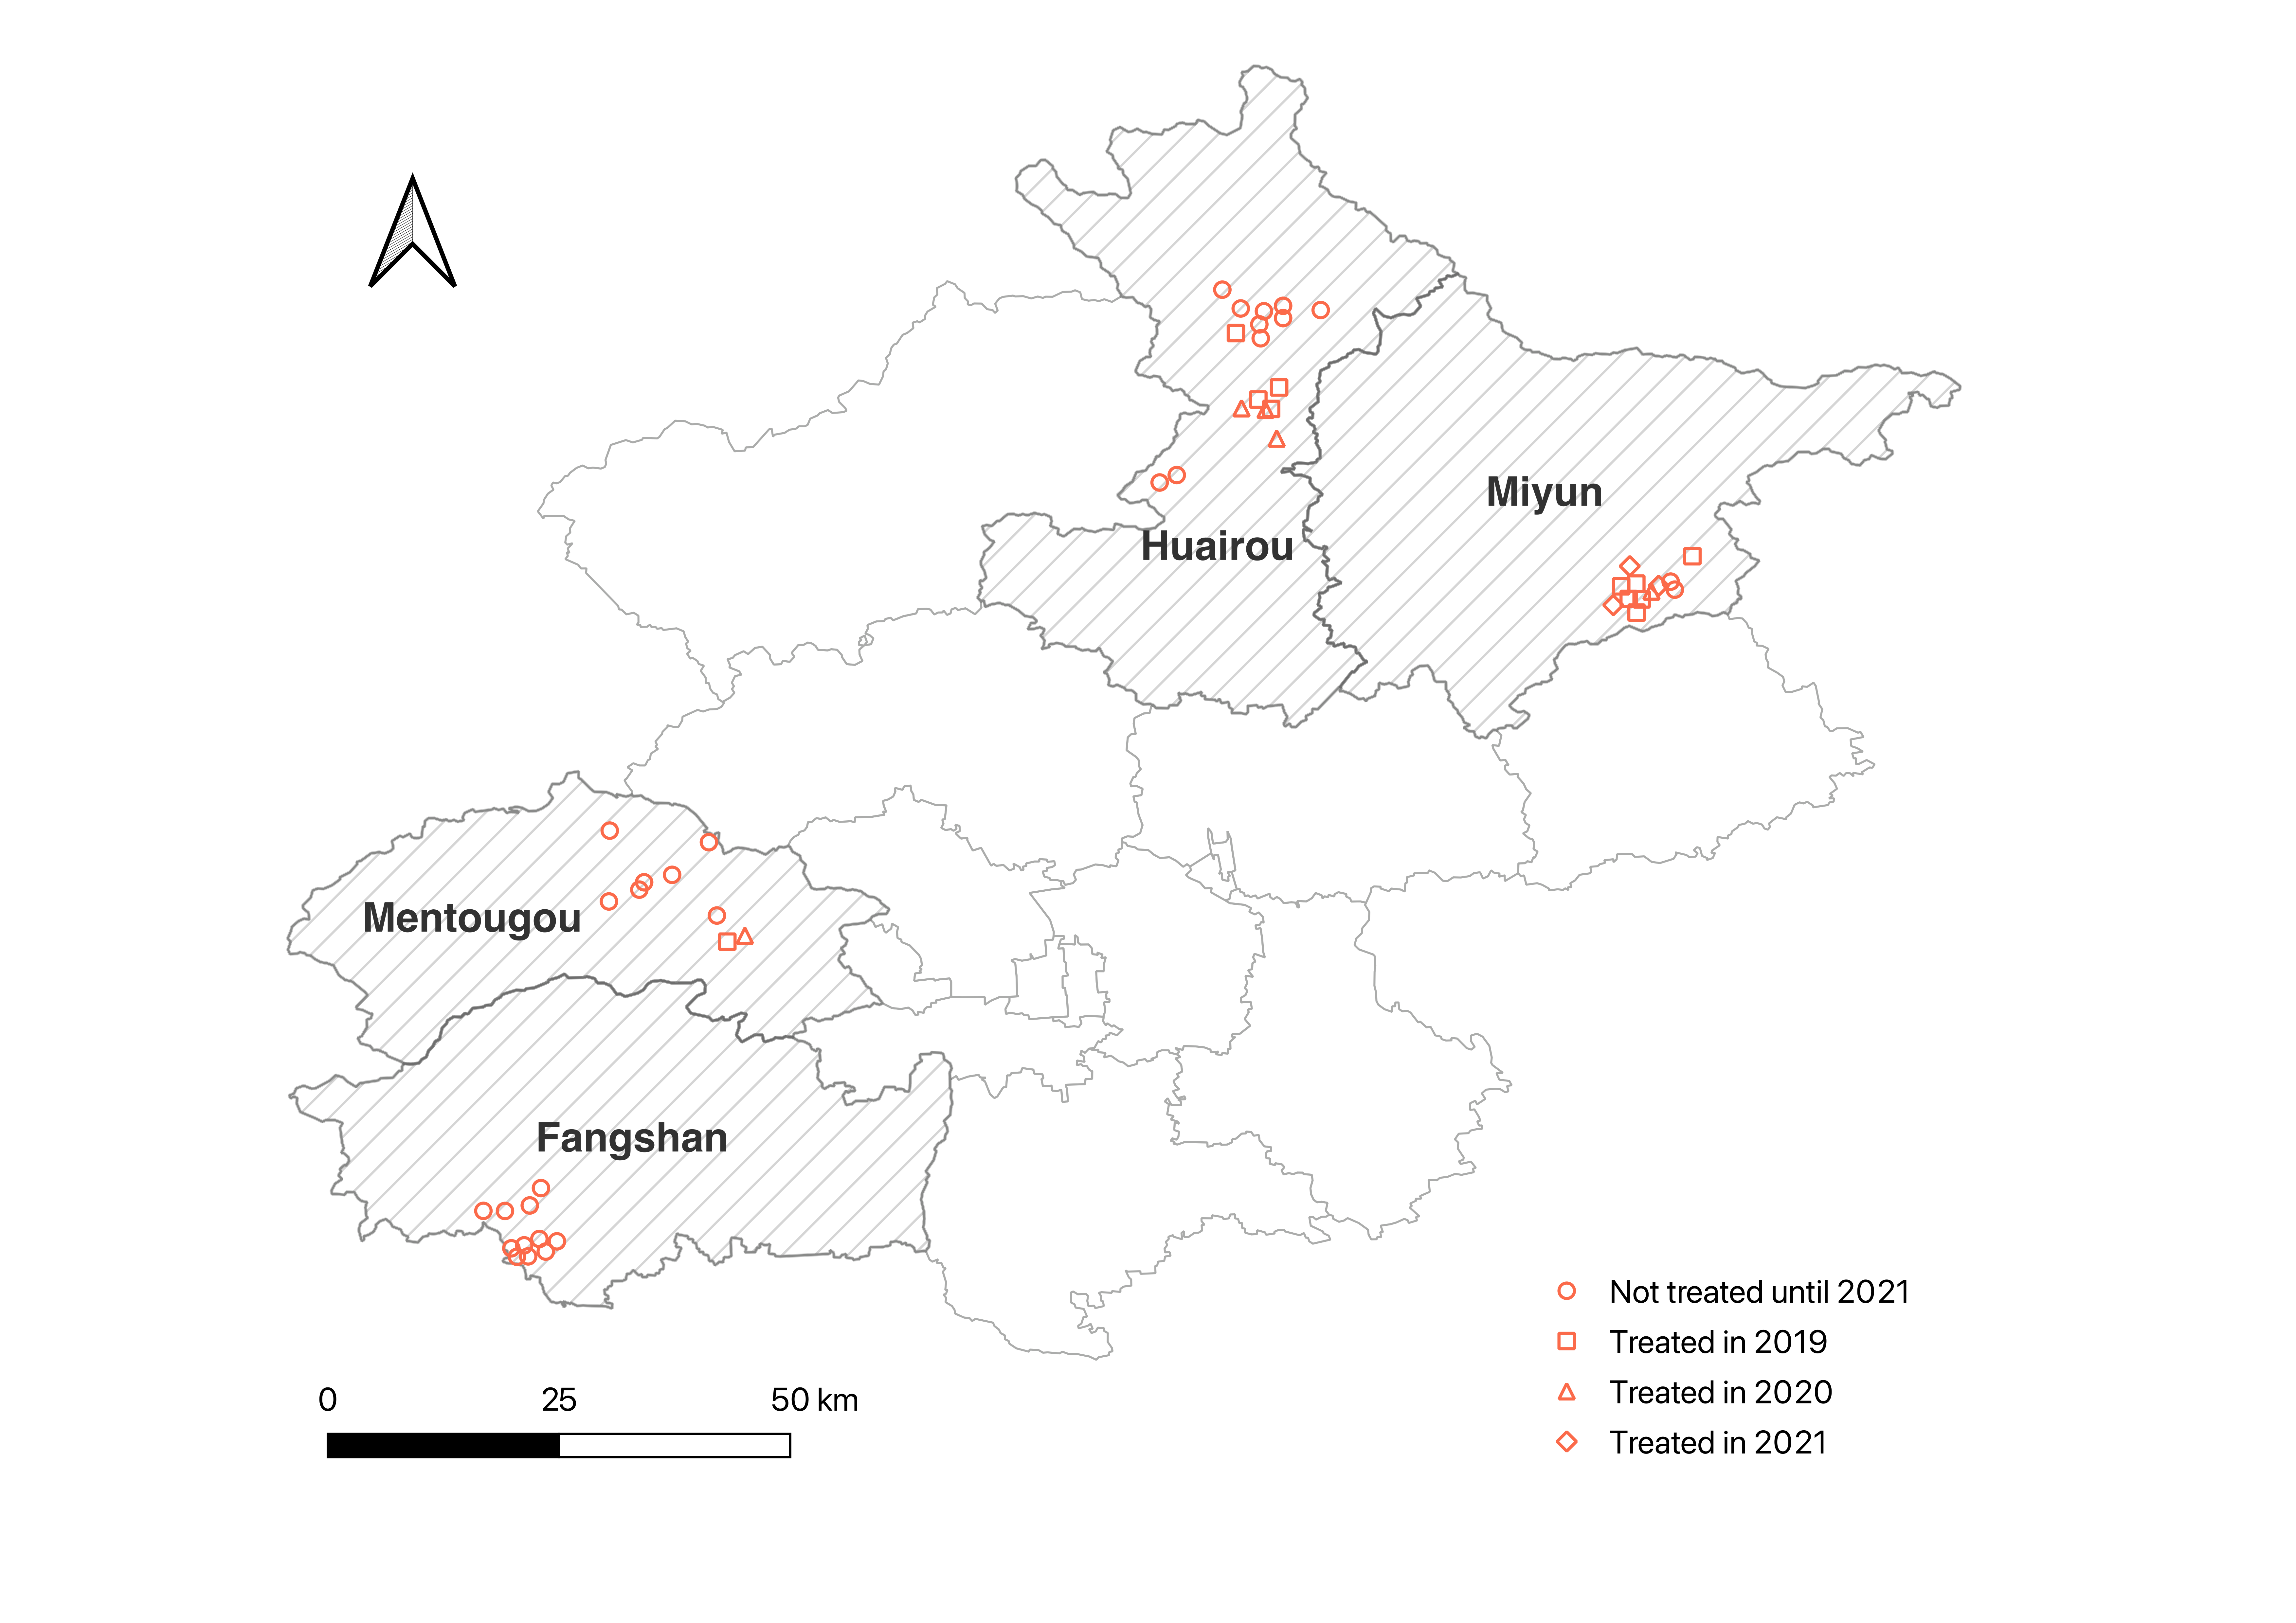
\includegraphics[width=0.5\textwidth,height=\textheight]{images/policy-implementation-map.png}

}

\caption{\label{fig-map1}Map of village implementation of CBHP policy}

\end{figure}

See Figure~\ref{fig-map1}.

\newpage

The source profiles for the four-factor solution are presented in Figure
X. The first source was identified as dust by high percentages of
crustal elements like wi-Ca, Si, and wi-Mg. The second source was
constituted of non-sulfate sulfur as well as secondary inorganic ions
(ammonium, nitrate, and sulfate). Non-sulfate sulfur is a tracer for
primary coal combustion, while secondary inorganic ions indicate a
secondary source. Since coal combustion is a major source of energy in
our study area, it is likely that the second source is a mixture of
primary and secondary emissions that originate from coal and other
sulfurous fuel combustion.

\begin{wrapfigure}{R}{0.7\textwidth}
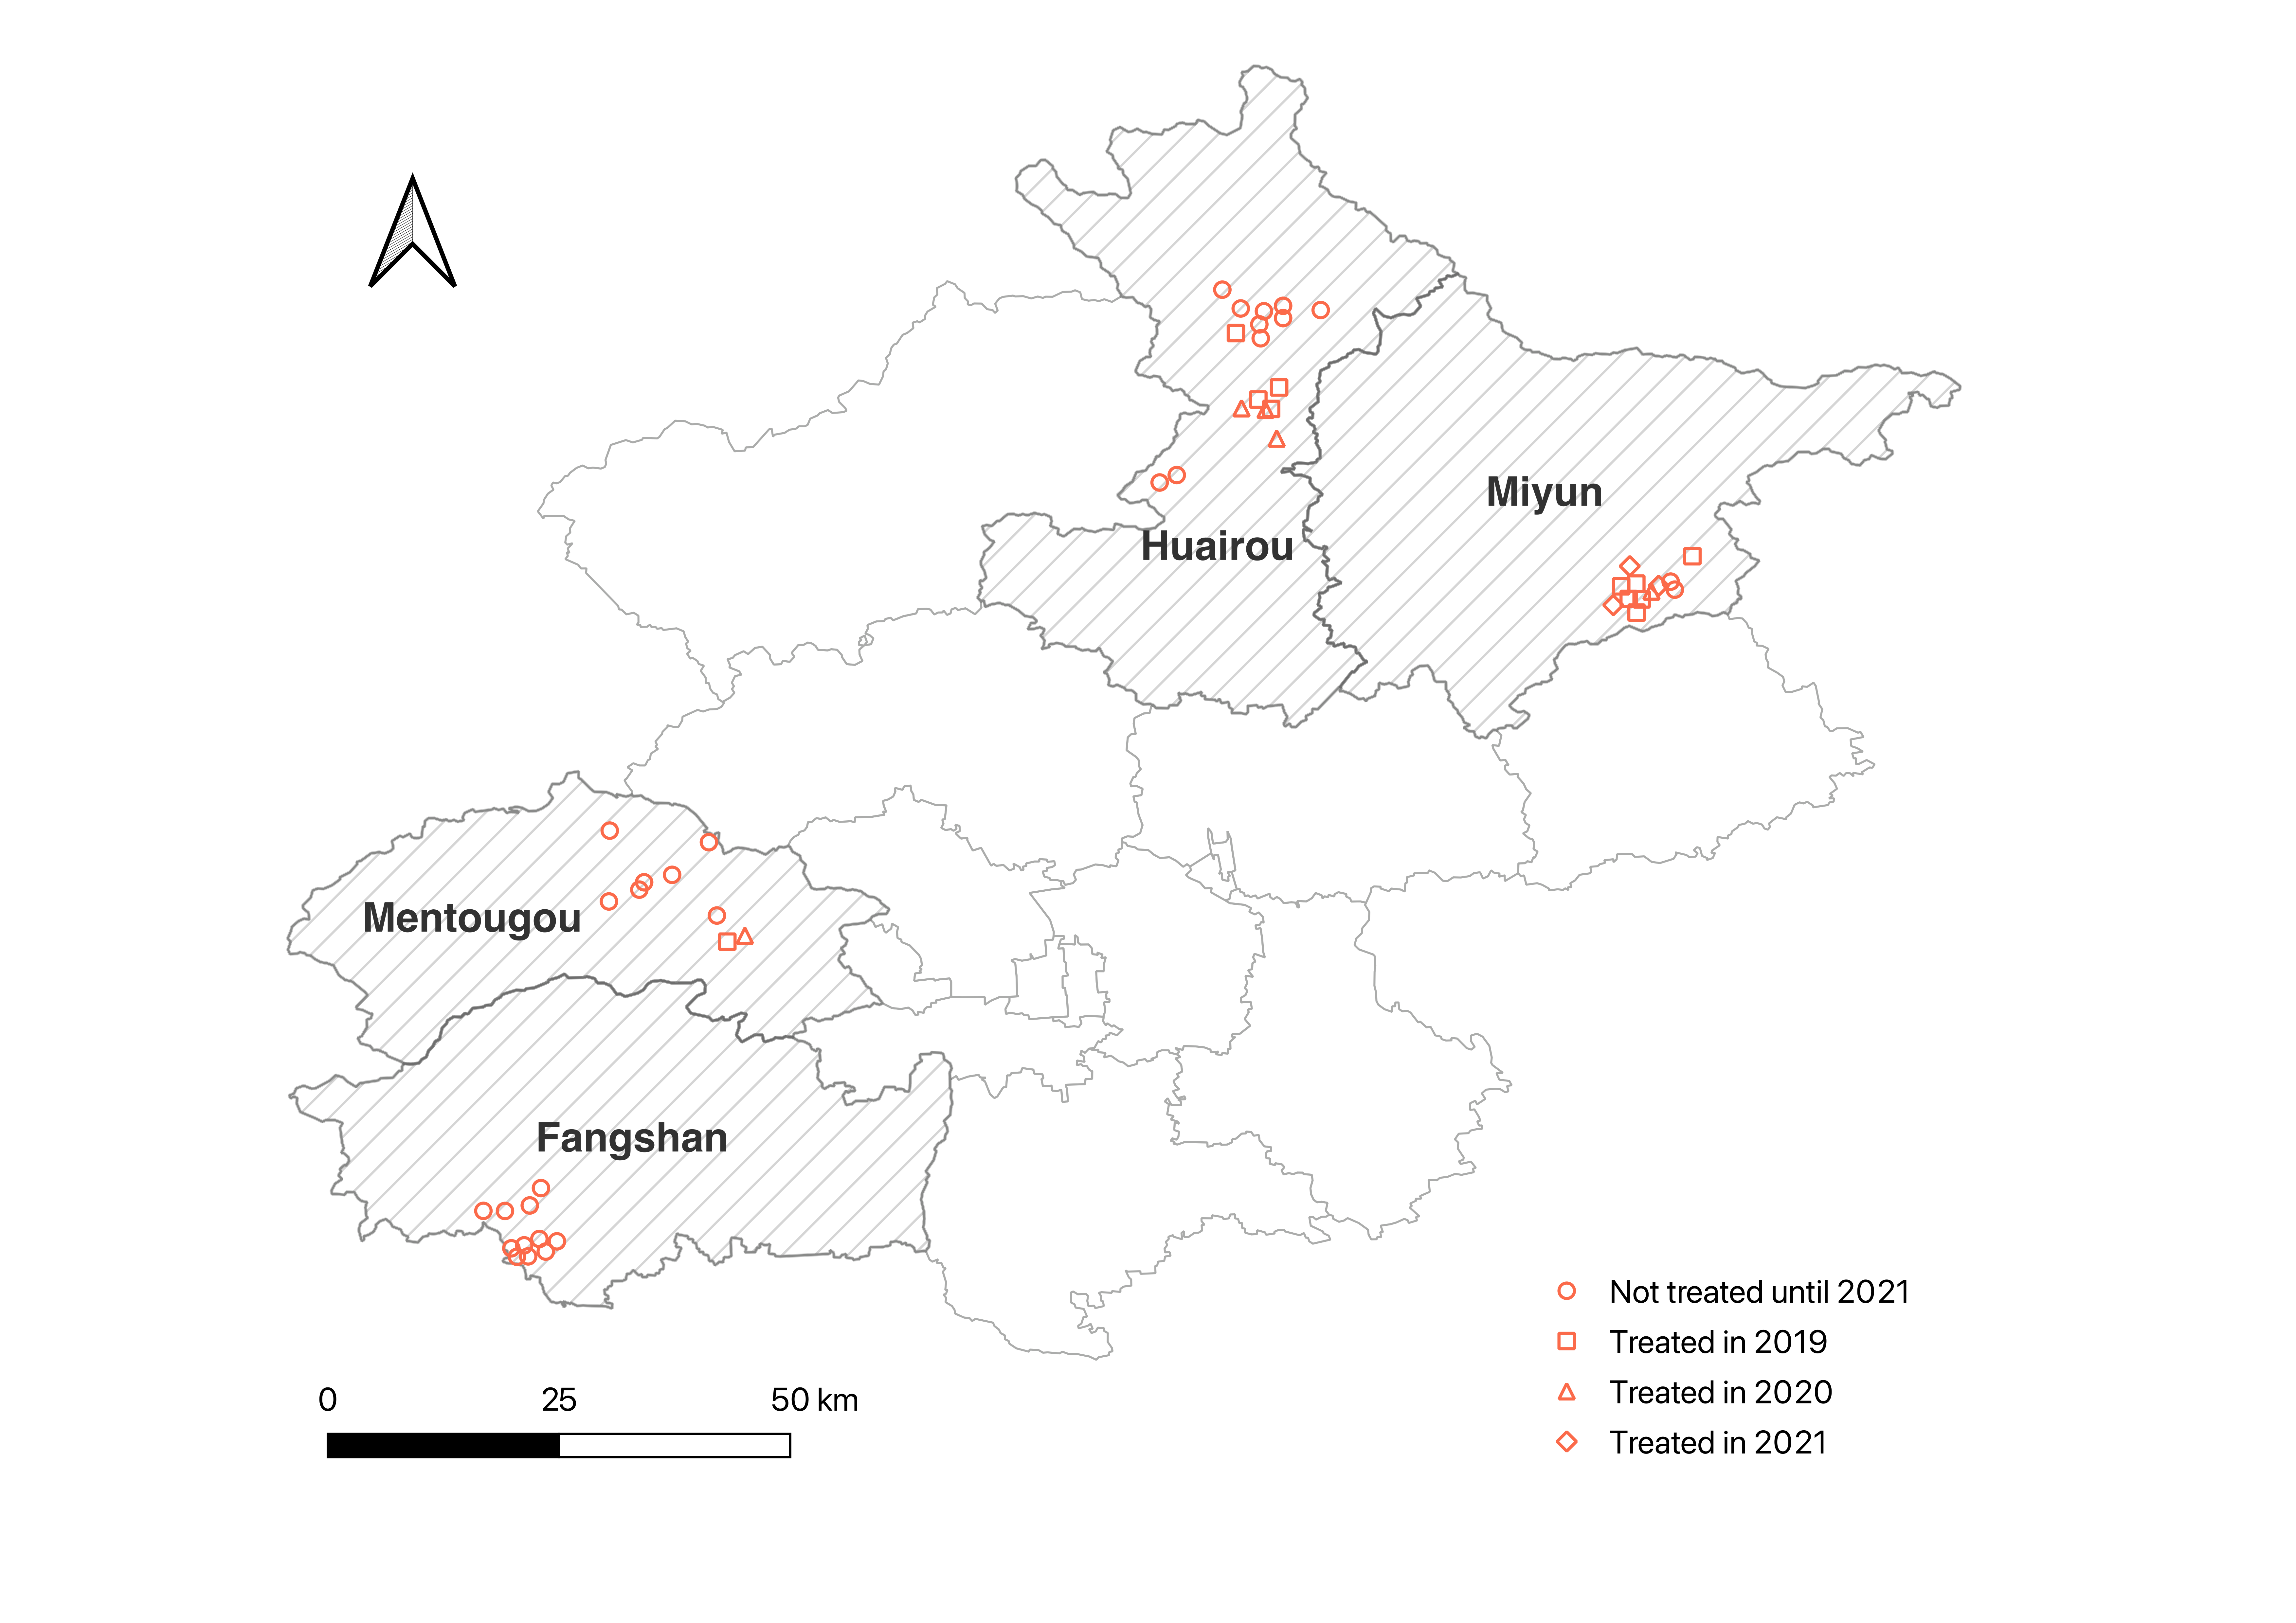
\includegraphics[width=0.7\textwidth]{images/policy-implementation-map.png}
\caption{\label{fig-map}{Google scholar metrics}}
\end{wrapfigure}

Additionally, in Figure\ref{fig-map} for details. the mean source
contribution of the second source is higher in outdoor than personal
exposure measurements. Secondary formation occurs outdoors in the
presence of sunlight, so higher outdoor concentrations compared to
personal exposure further support our naming the second source and
sulfur secondary. The third source had high percentages of ws-Ca nd Al,
which in our study region, has been found to be indicative of
transported dust from dust storms that can occur in the spring. While
our samples were collected during winter months only, it is possible
that transported dust from previous years still remained. The fourth
source was characterized by high percentages of tracers for both coal
(OC, wi-K, chloride, Pb) and biomass combustion (EC, ws-K). Coal and
biomass combustion is common in our study setting so this source is
likely a mixture of the two combustion sources.



\end{document}
